% =====================================================================
% Clase -- Geometría 4° -- Trimestre I -- Semana 04
% Sesión 004 (mié 23 sep., 8:40, 50 min)
% Tema: Líneas · Subtema: Rectas paralelas, secantes y perpendiculares
% Hilo conductor del trimestre I: «La vuelta al mundo en 80 días»
% Tema 1 de la guía: Líneas (tema:lineas)
% Material del docente (no se entrega a los estudiantes).
% =====================================================================
\documentclass[11pt]{article}
\makeatletter\def\input@path{{../../../../../plantillas/estilo/}}\makeatother
\usepackage{mmcantillo}
\guiadelestudiante{../../guia-didactica/guia-periodo-I-lineas-y-poligonos}

\tipodocumento{Clase}
\asignatura{Geometría}
\titulo{Semana 4: los rieles del tren}
\grado{4°}
\periodo{I}

% DBA: sin DBA propio. Las rectas paralelas y perpendiculares no están nombradas en los DBA
% de 4° (vienen del DBA 7 de 2°); aquí se trabajan como herramienta para describir figuras,
% que es el DBA 6 de 4° («Identifica, describe y representa figuras bidimensionales y
% tridimensionales, y establece relaciones entre ellas») y se usa en los temas 2 y 3. Está
% anotado en PENDIENTES.md como decisión abierta de la docente.

\begin{document}

\encabezado*

\begin{center}
{\renewcommand{\arraystretch}{1.3}
\begin{tabularx}{\linewidth}{@{}l l l X l@{}}
  \toprule
  \textbf{Sesión} & \textbf{Fecha} & \textbf{Min} & \textbf{Subtema} & \textbf{Entregables}\\
  \midrule
  004 & mié 23 sep., 8:40 & 50 & Rectas paralelas, secantes y perpendiculares & Taller\\
  \bottomrule
\end{tabularx}}
\end{center}

Segundo paso del hilo. Fogg sale de Londres en tren, y la vía por la que va es la mejor figura
que existe para esta clase: dos rieles que nunca se encuentran y unos durmientes que los cruzan
en escuadra. Referencia: \refguia{tema:lineas}.

% ---------------------------------------------------------------------
\seccion{Sesión 004 — miércoles 23 de septiembre · 8:40 · 50 min}

\textbf{Objetivo.} Reconocer y trazar rectas paralelas, secantes y perpendiculares, y
distinguirlas con un criterio, no de vista.

\textbf{Materiales.} Tablero; regla y escuadra (una por estudiante si se puede, o compartidas);
hoja cuadriculada. Si hay una foto o un dibujo de una vía de tren, mejor.

\begin{center}
{\renewcommand{\arraystretch}{1.3}
\begin{tabularx}{\linewidth}{@{}l l X@{}}
  \toprule
  \textbf{Momento} & \textbf{Min} & \textbf{Actividad}\\
  \midrule
  Enganche & 0--7 & «¿Por qué el tren no se sale de la vía?» Dibujar los dos rieles en el
    tablero y preguntar qué pasaría si se fueran juntando. Los rieles son paralelos: van
    siempre a la misma distancia y nunca se tocan, por más que se prolonguen.\\
  Tres parejas & 7--22 & Nombrar las tres relaciones con dibujos grandes: \textbf{paralelas}
    (no se cortan nunca), \textbf{secantes} (se cortan) y \textbf{perpendiculares} (se cortan
    formando la esquina de la escuadra: cuatro ángulos rectos). Los durmientes son
    perpendiculares a los rieles. La definición de Euclides, dicha con palabras de ellos:
    «prolongadas, no se encuentran».\\
  Trazar & 22--35 & Con regla y escuadra: cómo trazar una paralela a una recta dada (deslizar
    la escuadra apoyada en la regla) y cómo trazar una perpendicular (apoyar el lado corto de
    la escuadra). Que cada uno lo haga dos veces en la hoja cuadriculada.\\
  Taller & 35--47 & Taller individual (5 puntos).\\
  Cierre & 47--50 & Recoger. Anuncio: la próxima clase, figuras hechas con estas rectas —
    los polígonos.\\
  \bottomrule
\end{tabularx}}
\end{center}

\textbf{Figura para el tablero: la vía del tren.}

\begin{center}
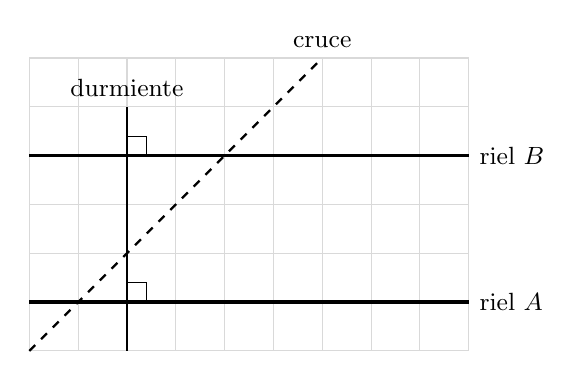
\begin{tikzpicture}[scale=0.62, every node/.style={font=\small}]
  \draw[gray!30] (0,-1) grid (9,5);
  \draw[very thick] (0,0) -- (9,0) node[right] {riel $A$};
  \draw[very thick] (0,3) -- (9,3) node[right] {riel $B$};
  \draw[thick] (2,-1) -- (2,4) node[above] {durmiente};
  \draw[thick, dashed] (0,-1) -- (6,5) node[above] {cruce};
  \draw (2,0) rectangle (2.4,0.4);
  \draw (2,3) rectangle (2.4,3.4);
\end{tikzpicture}

{\small Los cuadritos marcan los ángulos rectos. El cruce corta los rieles, pero no en
escuadra: es secante.}
\end{center}

\begin{nota}
\textbf{El error de siempre.} «No se tocan, entonces son paralelas.» Dos segmentos cortos
pueden no tocarse y aun así sus rectas cortarse al prolongarlas. La prueba es la regla: se
prolongan y se mira. Es la pregunta 3 del taller y conviene hacerla en el tablero si alguien
se atasca.
\end{nota}

\begin{nota}
\textbf{Sobre el DBA.} Paralelas y perpendiculares no aparecen en los DBA de 4° (vienen del
DBA 7 de 2°). Aquí se usan como herramienta para describir los cuadriláteros del tema 3, que sí
es DBA 6 de 4°. Es una de las decisiones que siguen abiertas en \texttt{PENDIENTES.md}.
\end{nota}

\end{document}
